\documentclass[crop,tikz]{standalone}% 'crop' is the default for v1.0, before it was 'preview'
\usepackage{amsmath}
\usepackage{amssymb }
%\usetikzlibrary{\ldots}
\usetikzlibrary{spy}
\usetikzlibrary{math}
\usetikzlibrary{intersections,calc,arrows,arrows.meta,decorations.pathreplacing}
\begin{document}

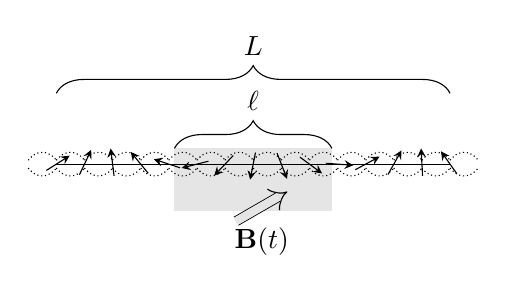
\begin{tikzpicture}


% Width
\def\w{5}

% Vertical offset for L label
\def\voL{0.9}
% Vertical offset for l label
\def\vol{0.2}
% Greyed-out area runs from width fraction f -> 1-f 
\def\f{0.3}
% Golden ratio for incommensurate spin rotation angles
\def\phi{ {(1+sqrt(5))/2} }

% Number of spins
\def\n{15}
% Length spin vector arrows
\def\arrowlength{0.3}

% Grey box for magnetic field (draw first so on bottom layer)
\fill[gray!20] ({\f*\w},-0.6) -- ({(1-\f)*\w},-0.6) -- ({(1-\f)*\w},0.2) -- (\f*\w,0.2) -- cycle;

% Axis line
\draw (0,0) -- (5,0);


% Draw interaction lines for final spin
\tikzmath{
   \pos = (-1)/(\n-1);
   \posph = (-0.5)/(\n-1);
   \posp = (0)/(\n-1);
}

\draw[densely dotted] plot [smooth,tension=1.1] coordinates {(\w*\pos,0.05) (\w*\posph,0.15)  (\w*\posp,0.05)};
\draw[densely dotted] plot [smooth,tension=1.1] coordinates {(\w*\pos,-0.05) (\w*\posph,-0.15)  (\w*\posp,-0.05)};

\foreach \x in {1,...,\n}{
   %Generate pseudorandom angle by using golden ratio
   \tikzmath{
      \pos = (\x-1)/(\n-1);
      \posph = (\x-0.5)/(\n-1);
      \posp = (\x)/(\n-1);
      \phix = \phi*\x;
   }
   %\filldraw ({\w*\pos} ,0) circle (0.1) node [above] {\x};
   % Draw interaction lines
   \draw[densely dotted] plot [smooth,tension=1.1] coordinates {(\w*\pos,0.05) (\w*\posph,0.15)  (\w*\posp,0.05)};
   \draw[densely dotted] plot [smooth,tension=1.1] coordinates {(\w*\pos,-0.05) (\w*\posph,-0.15)  (\w*\posp,-0.05)};
   % Draw spin vector arrow
   \draw[-stealth] ({\w*\pos} ,0)+(20*\phix:-\arrowlength/2) -- +(20*\phix:2*\arrowlength/3);
}

% \ell brace and label
\draw [decorate,decoration={brace,amplitude=10pt}] ({\w*\f},\vol) -- node[above,yshift=10]{$\ell$} ({\w*(1-\f)},\vol);

% Dotted delimeters for system proper
%\draw [densely dotted] ({\w*\f},-2*\vol) -- +(0,3*\vol);
%\draw [densely dotted] ({\w*(1-\f)},-2*\vol) -- +(0,3*\vol);

% B field symbol
\def\bl{0.5};
\draw [arrows={-Implies},double, double distance=1mm] (\w/2, -3*\vol) + (30:{-\bl/2}) -- node [below,yshift=-4] {${\bf B}(t)$} + (30:\bl);
\draw [color=gray!20, line width=1.05mm] (\w/2, -3*\vol) + (30:{-1.01*\bl/2}) -- + (30:0.756*\bl);

% L brace and label
\draw [decorate,decoration={brace,amplitude=10pt}] (0,\voL) -- node[above,yshift=10]{$L$} (\w,\voL);

\end{tikzpicture}
\end{document}
